\chapter{Princípy hardvérových MITM útokov}
\label{kap:principy}
V tejto kapitole stručne vysvetlíme základné princípy hardvérového MITM útoku a~spomenieme niektoré príklady známych útokov \cite{mitmSmartphone, mitmTouch, mitmTPM, mitmBitlocker, mitmI2C}. Následne opíšeme z toho vychádzajúcu motiváciu a ciele práce.

\section{Hardvérové útoky}
Útoky na hardvérovej úrovni, zneužívajú zraniteľnosti na fyzickom hardvéri daného zariadenia. Zraniteľnosti, ktoré umožňujú realizovať hardvérový útok je pomerne náročné opraviť, nakoľko je často potrebná výmena hardvéru, ktorá môže vyžadovať netriviálne náklady. Z hľadiska spôsobu zneužitia zraniteľností možno takéto útoky rozdeliť do dvoch kategórií.

\textbf{Pasívne} útoky sú založené na zraniteľnostiach, ktorých zneužitie si nevyžaduje fyzickú modifikáciu na danom hardvéri. Častým prípadom pasívnych útokov sú napríklad útoky s využitím postranných kanálov, napríklad rôzne útoky na hardvérové implementácie kryptografických primitív \cite{hwSec}.

\textbf{Aktívne} útoky si vyžadujú fyzický prístup k hardvéru, keďže ich princíp spočíva v~modifikácii vybraných hardvérových komponentov, pripadne iných faktorov fyzického prostredia, čo ovplyvňuje správanie hardvéru cieleným spôsobom. Príkladom sú útoky, ktoré využívajú zmenu napätia, elektromagnetické rušenie, výmenu hardvérových súčiastok a pod. \cite{hwSec}. Výhodou takéhoto útoku sú takmer neobmedzené možnosti ako ovplyvniť správanie hardvéru, čo poskytuje veľkú flexibilitu.

\section{Man-in-the-middle útoky}
Man-in-the-middle (MITM) je spôsob útoku na komunikáciu prebiehajúcu po kanáli medzi dvoma entitami, pri ktorom útočník presmeruje komunikáciu z pôvodného kanálu na druhý kanál, ktorý je pod kontrolou útočníka. Takýto útok je často realizovaný transparentne z pohľadu účastníkov komunikácie a vytvára tým zdanie, že účastníci sú spojený priamo. V skutočnosti však komunikácia prechádza cez tretiu entitu, ktorú má útočník pod kontrolou (napr. zariadenie, proces, systém). Tá je následne schopná, komunikáciu či už pasívne odpočúvať, alebo dokonca aktívne do komunikácie zasahovať. Schéma MITM útoku je znázornená na obrázku \ref{obr:mitm}.

\begin{figure}
    \centerline{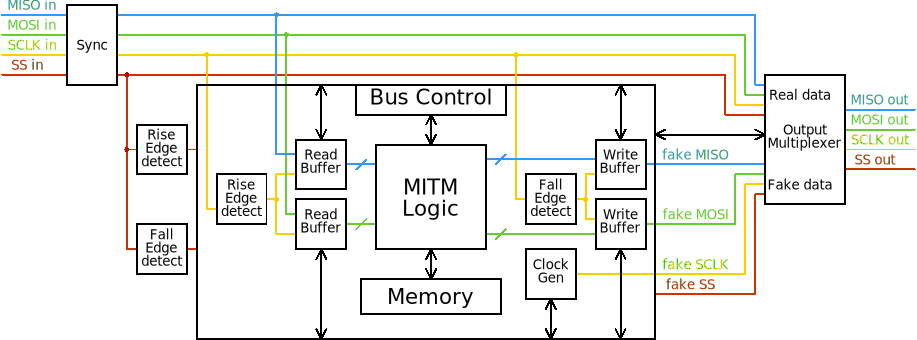
\includegraphics[width=0.75\textwidth]{images/mitm.png}}
    \caption[Schéma MITM útoku]{Schéma MITM útoku.}
    \label{obr:mitm}
\end{figure}

Opatrení, ktoré znemožňujú týmto spôsobom útočiť na komunikáciu je viacero, ich princíp sa však opiera o tri základné požiadavky informačnej bezpečnosti. Zabezpečujú dôvernosť prenášanej informácie pre znemožnenie pasívneho odpočúvania, integritu a~autenticitu za účelom znemožnenia aktívneho zasahovania do komunikácie, prípadne aj detekciu pokusu o MITM útok \cite{mitmTheory}. 

\section{Hardvérové MITM útoky}
MITM útoky sú často uvažované v prostredí sieťovej komunikácie, kde má útočník prístup k niektorému zo zariadení alebo procesov podieľajúcich sa na prenose informácie po sieti, napr. smerovač (angl. router) \cite{mitmTheory}. MITM útok je však oveľa všeobecnejší a jeho techniku možno aplikovať prakticky v akomkoľvek scenári, kde prebieha komunikácia medzi dvoma entitami.

Zaujímavou myšlienkou, ktorá využíva MITM princíp je útok na komunikáciu prebiehajúcu po zbernici medzi jednotlivými hardvérovými komponentami. Príkladom takéhoto útoku môže byť ovplyvnenie komunikácie medzi CPU a pamäťou. Dôležitý predpoklad je prístup ku kanálu (alebo aspoň jeho časti), po ktorom prebieha komunikácia, teda v tomto prípade fyzický prístup ku zbernici. Tento predpoklad je pomerne silný a~preto sa bezpečnosť komunikácie po zbernici častokrát zanedbáva a uprednostňuje sa funkcionalita a jednoduchosť implementácie.

Pri bežných systémoch ako sú napríklad osobné počítače, pracovné stanice, či servery je fyzický prístup útočníka menej pravdepodobný, resp. zvyknú byť implementované iné opatrenia pre jeho zabránenie. Vnorené (angl. embedded) systémy sa čoraz viac využívajú na ovládanie rôznych inteligentných zariadení ako napríklad inteligentné zámky, inteligentné domáce spotrebiče a pod. Tieto zariadenia tiež obsahujú množstvo rôznych integrovaných obvodov, ktoré navzájom komunikujú po zberniciach.

V prípade takýchto zariadení je predpoklad fyzického prístupu útočníka často naplnený. Potenciálnym útočníkom môže byť v takomto prípade aj samotný používateľ, ktorého cieľom môže byť obísť mechanizmus implementovaný výrobcom, s cieľom obmedziť použitie, resp. modifikáciu daného zariadenia (napr. vendor lock-in). V ďalšej časti predstavíme niekoľko známych útokov z iných prác, s cieľom poukázať na možnosti hardvérového MITM útoku a dôležitosť ochrany komunikácie po zberniciach.

\section{Príklady známych hardvérových MITM útokov}
Existuje viacero prác, ktoré sa zaoberali hardvérovými MITM útokmi \cite{mitmSmartphone, mitmTouch, mitmTPM, mitmBitlocker, mitmI2C}. Prvým zaujímavým útokom, ktorý spomenieme je útok na odomykací mechanizmus smartfónu \cite{mitmSmartphone}. Princíp útoku spočíva v ovplyvnení komunikácie medzi CPU a~externou stálou (angl. non-volatile) pamäťou, ktorá obsahovala údaje o zostávajúcom počte pokusov. Komunikácia medzi CPU a pamäťou bola síce šifrovaná, ale útok zneužíval fakt, že posielané správy neboli označené jedinečným identifikátorom, napríklad časovou pečiatkou \cite{mitmSmartphone}. To umožnilo vykonať útok opakovaním správy s informáciou o zostávajúcom počte pokusov, ktorá prichádzala z pamäte do CPU. Následne bolo možné vykonať útok hrubou silou -- úplným preberaním z množiny slov pevnej dĺžky nad desiatkovými číslicami.

Veľká časť smartfónov, tabletov, notebookov, či iných zariadení považuje hardvérové komponenty inštalované pri výrobe automaticky za dôveryhodné \cite{mitmTouch}. Takýto bezpečnostný prístup viedol k zaujímavému hardvérovému MITM útoku. Opäť išlo o~útok na smartfón, ktorý tentokrát výmenou dotykovej obrazovky za obrazovku úmyselne pripravenú útočníkom, umožnil vykonávať útočníkom kontrolované operácie nad príkazmi zadávanými používateľom do obrazovky. Náhradná obrazovka bola následne schopná pasívne odpočúvať vstup od používateľa, vykonávať operácie v mene používateľa a~dokonca zneužitím ďalších zraniteľností prítomných v jadre operačného systému získať administrátorské práva a tým aj úplnú kontrolu nad zariadením \cite{mitmTouch}. Autori zároveň poukazujú na realistický scenár tohto útoku, odvolávajúc sa na častú výmenu poškodených obrazoviek službami poskytovanými v neautorizovaných servisoch.

Ďalšia zaujímavá skupina útokov, sú útoky na externý TPM modul (Trusted Platform Module). TPM je hardvérový modul, ktorý poskytuje rôzne bezpečnostné funkcie. Jednou z nich je mechanizmus merania a ukladania tzv. udalostí \cite{tpmArch}, ktoré na danej platforme nastali. Tento mechanizmus sa využíva aj na kontrolu integrity programov spúšťaných pri štarte zariadenia. \uv{TPM Reset Attack} je útok, ktorý resetovaním TPM modulu umožňuje obísť spomenutú kontrolu integrity \cite{mitmTPM}. TPM ďalej poskytuje možnosť generovania náhodných čísel s vysokou entropiou \cite{tpmArch}. Existuje útok na TPM modul, ktorý zneužíva fakt, že TPM protokol nezabezpečuje autentickosť správy, ktorá obsahuje náhodne vygenerované dáta. Útočník, teda môže zasiahnuť do komunikácie a ľubovoľne modifikovať vygenerované dáta \cite{mitmTPM}. Spomenuté útoky predpokladajú externý TPM modul a nie sú aplikovateľné v prípade, že TPM je integrovaný priamo na čipe s procesorom.

Ďalšie príklady hardvérových MITM útokov sú pasívneho charakteru \cite{mitmI2C, mitmBitlocker}. Tieto útoky zneužívajú nezabezpečenú dôvernosť komunikácie po zberniciach a zameriavajú sa preto na odpočúvanie komunikácie. Najčastejším príkladom takýchto útokov je odpočúvanie dôvernej informácie ako napríklad kryptografických kľúčov, ktoré môžu tiecť po zbernici napr. medzi CPU a spomínaným TPM modulom. Takéto údaje zvyknú byť bezpečne uložené v špecializovaných integrovaných obvodoch. Odpočúvanie komunikácie na zbernici je preto často značne jednoduchší spôsob získania týchto údajov ako priama manipulácia s čipom obsahujúcim dané údaje \cite{mitmBitlocker}.

Všetky tieto útoky zneužívajú fakt, že pri návrhu komunikácie medzi hardvérovými komponentami sa často očakáva dôveryhodné prostredie (zbernica), v ktorom komunikácia prebieha. Práce poukazujú aj na to, že v poslednej dobe je tento predpoklad čoraz zriedkavejšie pravdivý.

\section{Možné protiopatrenia}
Pri klasickom MITM scenári po sieti spočívajú protiopatrenia v zabezpečení integrity a~autentickosti prebiehajúcej komunikácie prostredníctvom kryptografie, napr. použitím TLS protokolu \cite{mitmTheory}. V hardvérovom scenári môže však takýto druh protiopatrení spôsobiť problém, z dôvodu obmedzenej výpočtovej kapacity. Nie všetky integrované obvody disponujú hardvérom, ktorý by bol schopný realizovať potrebné kryptografické operácie. Pri zariadeniach, ktoré v rámci hardvéru obsahujú aj procesor so všeobecnejšou inštrukčnou sadou je možné takéto protiopatrenie implementovať na úrovni firmvéru. Napriek tomu sa ich implementácia často zanedbáva.

Navyše, štandardy pre prenos dát po vysokorýchlostných zberniciach (napr. PCIe, USB 3.0) špecifikujú pomerne veľké rýchlosti prenosu, rádovo od Mb/s až po desiatky Gb/s \cite{pcieSpec, usbSpec}. To znamená, že navrhnuté protiopatrenie musí umožniť dostatočne rýchle spracovanie správy, ktoré bude v súlade so štandardom. Niekedy to môže znamenať potrebu spracovať správu rádovo za niekoľko mikrosekúnd až nanosekúnd.

Iná možnosť môže byť napr. implementovať opatrenia pre zabezpečenie dôvernosti, integrity a autentickosti komunikácie na vyššej vrstve. Napríklad komunikácia medzi CPU a pamäťou, alebo iným úložným priestorom, môže byť zabezpečená priamo na CPU, ktoré môže šifrovať/podpisovať dáta pred zápisom a dešifrovať/overovať podpis dát po následnom prečítaní. Tento prístup bol čiastočne, no ako autori poukázali nedostatočne, implementovaný pri útoku na odomknutie smartfónu \cite{mitmSmartphone}, spomenutom v~predošlej časti.

\section{Motivácia a ciele práce}
V spomenutých prácach sú jednotlivé útoky implementované a analyzované pre konkrétne zbernice. Tieto zbernice majú odlišné vlastnosti na fyzickej vrstve, ktoré podrobnejšie rozoberieme v kapitole \ref{kap:zbernice}. Niektoré útoky, napr. spomenuté útoky na TPM, zneužívajú zraniteľnosti protokolu na vyššej vrstve, napr. nedostatočná kontrola integrity prenášaných správ. Z pohľadu MITM logiky útoku v takomto prípade nie je relevantná fyzická vrstva danej zbernice.

Cieľom práce je preto preskúmať do akej miery je možné oddeliť fyzickú vrstvu zbernice od logiky operácií nad komunikáciou, ďalej len MITM logiky. V kapitole \ref{kap:implementacia} navrhneme implementáciu FPGA obvodu, ktorý bude realizovať vybrané MITM operácie nad komunikáciou. Spôsob implementácie umožní oddeliť niektoré aspekty fyzickej vrstvy zbernice a~nezávisle od seba zamieňať implementáciu konkrétnej zbernice a~MITM logiky. Zároveň poukážeme na niektoré principiálne neabstrahovateľné vlastnosti spôsobené asymetrickou tzv. master-slave architektúrou, ktorú bližšie popíšeme v kapitole \ref{kap:zbernice}.

\subsection{Relevantné operácie nad komunikáciou}
Identifikovali sme aj niektoré relevantné operácie nad komunikáciou, ktoré môžu byť užitočné pri hardvérových MITM útokoch. Užitočnou operáciou MITM útoku môže byť nahradenie vybraných príznakov v statusových alebo konfiguračných správach. Takýmto spôsobom možno ovplyvniť niektoré bezpečnostné nastavenia, napríklad zakázanie zápisových operácií do pamäte. Iným príkladom môže byť napríklad falšovanie stavu, že obvod ešte nie je pripravený na ďalšiu komunikáciu, s cieľom získať čas na potrebné výpočty nad predošlou komunikáciou. Pri nahrádzaní takýchto príznakov je často postačujúca možnosť vykonávať bitové operácie nad komunikáciou.

Ďalšou relevantnou operáciou je nahradenie dát, príp. časti dát za inú hodnotu. Táto hodnota môže byť konštanta, alebo aj premenná závislá napríklad od predošlej komunikácie, prípadne externého vstupu od používateľa. V prípade implementácie MITM logiky na FPGA môže byť preto užitočné implementovať aj pamäťový obvod, ktorý bude schopný uchovávať informácie o predošlej komunikácii a zároveň pridať možnosť vstupu od používateľa. Medzi operácie takéhoto typu možno taktiež zaradiť tzv. útoky opakovaním správy, kde nahradíme celú správu v rámci komunikácie za inú predošle odchytenú správu. Blokovanie komunikácie je ďalšou operáciou, ktorú môžeme považovať za nahradenie dát prázdnou správou, ktorá v závislosti od zbernicového protokolu môže znamenať, že daná strana skutočne pošle prázdnu správu (napr. konštantu 0), alebo komunikácia vôbec nebude inicializovaná.

Spomenuté operácie využijeme na konkrétnych príkladoch demonštrácie fungovania nášho FPGA obvodu. Existujú aj ďalšie operácie, ktoré v závislosti od konkrétneho scenára môžu byť užitočné, napríklad výpočet niektorej funkcie nad komunikáciou. Pre takéto operácie sme však neidentifikovali relevantný scenár, preto sa im v práci nebudeme venovať.